\section{Pianificazione}
Lo sviluppo del progetto è costruito sulla base delle scadenze riportate nella sottosezione \textsection1.5 ed è suddiviso nelle seguenti fasi:
\begin{itemize}
	\item analisi;
	\item consolidamento dei requisiti
	\item progettazione architetturale;
	\item progettazione di dettaglio e codifica;
	\item validazione e collaudo.
\end{itemize}

\subsection{Analisi}
\textbf{Periodo}: dal 2020-03-10 al 2020-04-13 \\
Questo periodo ha inizio con la formazione dei gruppi e termina con la scadenza per la consegna dei documenti relativi alla \textit{Revisione dei Requisiti}. \\
Le principali attività svolte in questo periodo sono:
\begin{itemize}
	\item \textbf{Strumenti di lavoro}: questa attività consiste nella scelta degli strumenti di lavoro da utilizzare per lo svolgimento del progetto;
	\item \textbf{\NdP{}}: attività nella quale gli Amministratori redigono le \textit{\NdP{}}, documento in cui si specificano tutte le regole, le convenzioni e le tecnologie che i componenti del gruppo adotteranno durante tutto il corso del progetto. Questa attività include una stesura iniziale del documento, comprensiva delle norme e degli standard accordati dal gruppo, il documento verrà poi ampliato in base all'individuazione di sezioni da integrare;
	\item \textbf{\SdF{}}: attività nella quale gli Analisti redigono lo \textit{\SdF}, documento in cui vengono analizzati i capitolati\ped{\textit{G}} d'appalto elencando per ciascuno i punti positivi e negativi che li caratterizzano. Inoltre vengono indicate le motivazioni per le quali è stato scelto il capitolato\ped{\textit{G}} C2 denominato \textit{Etherless} e sono stati esclusi i capitolati\ped{\textit{G}} restanti. \\
	Questa attività è bloccante per l'inizio dell'\textit{\AdR{}};
	\item \textbf{\AdR{}}: attività nella quale gli Analisti redigono l'\textit{\AdR{}}, documento essenziale in cui viene analizzato in maniera approfondita il capitolato\ped{\textit{G}} scelto a seguito dello \textit{\SdF}, individuando le funzionalità e i casi d'uso\ped{\textit{G}} previsti dal progetto;
	\item \textbf{\PdP{}}: attività nella quale il Responsabile redige il \textit{\PdP}, documento in cui viene presentata la pianificazione del gruppo per lo sviluppo del progetto, un'analisi dei rischi e dei costi e dove vengono indicate le scadenze che il gruppo intende rispettare per la buona riuscita del progetto;
	\item \textbf{\PdQ{}}: attività nella quale gli Analisti redigono il \textit{\PdQ}, documento in cui vengono indicate tutte le strategie di verifica e validazione che il gruppo intende adottare con lo scopo di garantire la qualità di processo e di prodotto\ped{\textit{G}};
	\item \textbf{\Glossario{}}: attività nella quale viene redatto il \textit{\Glossario}, documento nel quale verranno elencati, chiariti ed approfonditi tutti i termini tecnici utilizzati nei documenti con lo scopo di evitare possibili ambiguità;
	\item \textbf{Lettera di Presentazione}: attività nella quale viene redatta la \textit{Lettera di Presentazione} necessaria per la presentazione come fornitore del gruppo.
\end{itemize}
	\subsubsection{Diagramma di Gantt: Analisi}
		\begin{figure}[h]
			\centering
			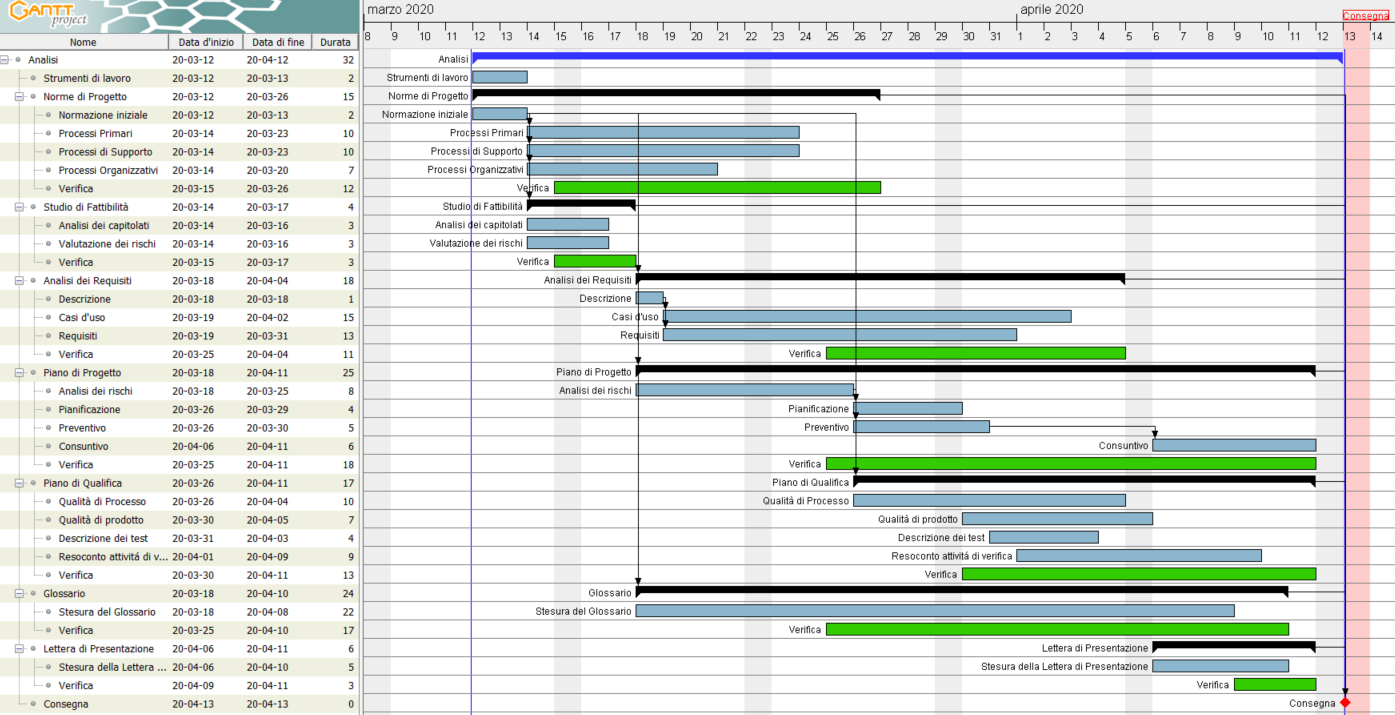
\includegraphics[width=1.1\textwidth]{./res/img/DiagrammiGantt/analisi_gantt.png}
			\caption{Diagramma di Gantt del periodo di Analisi}
		\end{figure}

\subsection{Consolidamento dei Requisiti}
\textbf{Periodo}: dal 2020-04-13 al 2020-04-20 \\
Questo periodo ha inizio dopo il termine del periodo di Analisi e termina il giorno della presentazione della \textit{Revisione dei Requisiti}. \\
\begin{itemize}
	\item \textbf{Incremento e Verifica dei documenti:} in caso di necessità, vengono migliorati e verificati i documenti preparati nel periodo precedente;
	\item \textbf{Consolidamento Analisi dei requisiti}: l'attività principale, prevede un consolidamento e un miglioramento dei requisiti ottenuti concluso il periodo di Analisi e conseguente aggiornamento dell'\textit{\AdR{}};
	\item \textbf{Realizzazione della presentazione:} preparazione del materiale necessario alla presentazione del 2020-04-20.
\end{itemize}
	\subsubsection{Diagramma di Gantt: Consolidamento dei Requisiti}
		\begin{figure}[h]
			\centering
			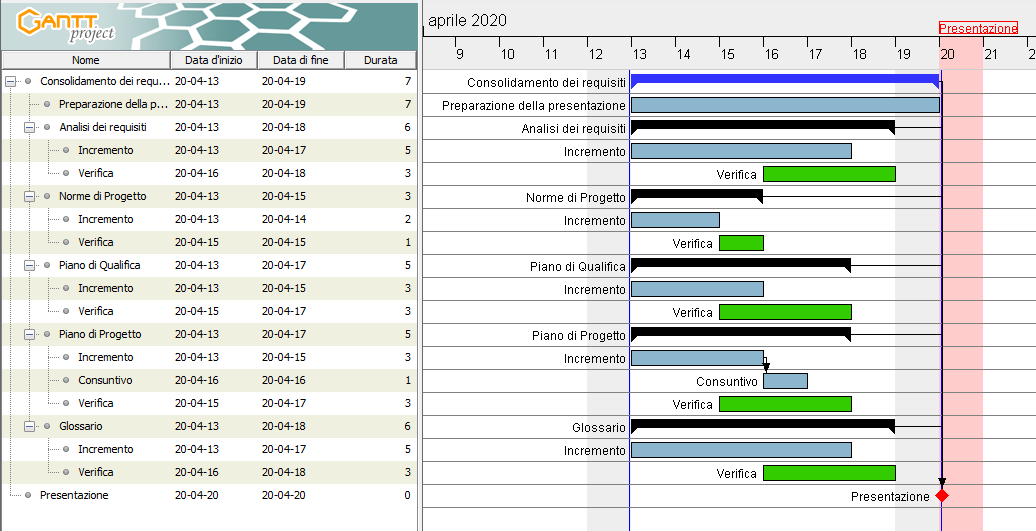
\includegraphics[width=1.1\textwidth]{./res/img/DiagrammiGantt/cons_req_gantt.png}
			\caption{Diagramma di Gantt del periodo di Consolidamento dei Requisiti}
		\end{figure}
\newpage

\subsection{Progettazione Architetturale}
\textbf{Periodo}: dal 2020-04-20 al 2020-05-18 \\
Questo periodo ha inizio al termine del periodo di Consolidamento dei Requisiti e termina alla \textit{Revisione di Progettazione}. \\
Questo periodo porta all'individuazione di una soluzione architetturale che permetta il soddisfacimento dei requisiti individuati.
\begin{itemize}
	\item \textbf{Incremento e verifica}: come prima cosa, analizzando l'esito della \textit{Revisione dei Requisiti} vengono svolte attività di incremento e verifica sui vari documenti redatti, dove necessario. \\
	L'incremento dell'\textit{\AdR{} 1.0.0} è il più importante perchè va completato prima di poter proseguire con il resto delle attività;
	\item \textbf{Technology Baseline}\ped{\textit{G}}: viene redatta la documentazione di supporto, contenente la descrizione delle tecnologie individuate e il tracciamento della relazione tra le componenti e i requisiti che vanno a soddisfare. Viene anche codificato il \textbf{PoC (Proof of Concept)} come dimostrazione del funzionamento dell'architettura individuata;
	\item \textbf{Glossario}: attività che prevede un miglioramento del \textit{\Glossario{} 1.0.0} aggiungendo nuovi termini oppure raffinando le definizioni di termini già presenti.
\end{itemize}
	\subsubsection{Incrementi}
		\subsubsubsection{Descrizione}
			\begin{itemize}
				\item \textbf{1$^{\circ}$ Incremento:} integrazione dei documenti a seguito delle conoscenze acquisite nei periodi precedenti;
				\item \textbf{2$^{\circ}$ Incremento:} implementazione della componente Etherless-smart;
				\item \textbf{3$^{\circ}$ Incremento:} implementazione della componenete Etherless-CLI\ped{\textit{G}}; \\
				Comandi da implementare per il PoC, legati ai requisiti che soddisfano:
					\rowcolors{2}{lightRowColor}{darkRowColor}
					\begin{longtable}{
						>{\centering}p{0.25\textwidth}
						>{\centering}p{0.20\textwidth} }

						\coloredTableHead
						\textbf{\color{white}Comando} &
						\textbf{\color{white}Requisiti}
						\tabularnewline
						\endhead

						\hline \multicolumn{2}{c}{\textit{Continua nella prossima pagina}} \\
						\endfoot
						\hline
						\endlastfoot
						signup & R1F3\\ R1F3.1 \\ R1F3.1.1 \\ R1F3.1.2 \\ R1F3.1.3\tabularnewline
						login & R1F4 \\ R1F4.1 \\ R1F4.1.1 \\ R1F4.1.2\tabularnewline
						logout & R1F5\tabularnewline
						run & R1F9 \\ R1F9.1 \\ R1F9.2 \\ R1F9.3\tabularnewline
						\rowcolor{white}\caption{Tracciamento comandi-requisiti soddisfatti}	\\

					\end{longtable}
				\item \textbf{4$^{\circ}$ Incremento:} implementazione della componente Etherless-server;
				\item \textbf{5$^{\circ}$ Incremento:} integrazione delle componenti sviluppate;
				\item \textbf{6$^{\circ}$ Incremento:} correzione della documentazione a seguito della correzione della RR e preparazione in vista della \TB{}\ped{\textit{G}};
				\item \textbf{7$^{\circ}$ Incremento:} ulteriori aggiornamenti della documentazione, con passaggio alla versione 2.0.0:
				\begin{itemize}
					\item consuntivo di periodo nel \PdP{};
					\item aggiornamento \NdP{} e \PdQ{};
					\item eventuali aggiornamenti riguardanti il \Glossario{}.
				\end{itemize}
				\item \textbf{8$^{\circ}$ Incremento:} preparazione della presentazione per la RP.
			\end{itemize}
		\subsubsubsection{Scadenze}
			\begin{itemize}
				\item \textbf{1$^{\circ}$ Incremento:} entro 2020-04-22;
				\item \textbf{2$^{\circ}$ Incremento:} entro 2020-04-24;
				\item \textbf{3$^{\circ}$ Incremento:} entro 2020-04-26;
				\item \textbf{4$^{\circ}$ Incremento:} entro 2020-04-27;
				\item \textbf{5$^{\circ}$ Incremento:} entro 2020-04-28; % 29???
				\item \textbf{6$^{\circ}$ Incremento:} entro 2020-05-04;
				\item \textbf{7$^{\circ}$ Incremento:} entro 2020-05-11;
				\item \textbf{8$^{\circ}$ Incremento:} entro 2020-05-18.
			\end{itemize}

	\subsubsection{Diagramma di Gantt: Progettazione Architetturale}
		\begin{figure}[h]
			\centering
			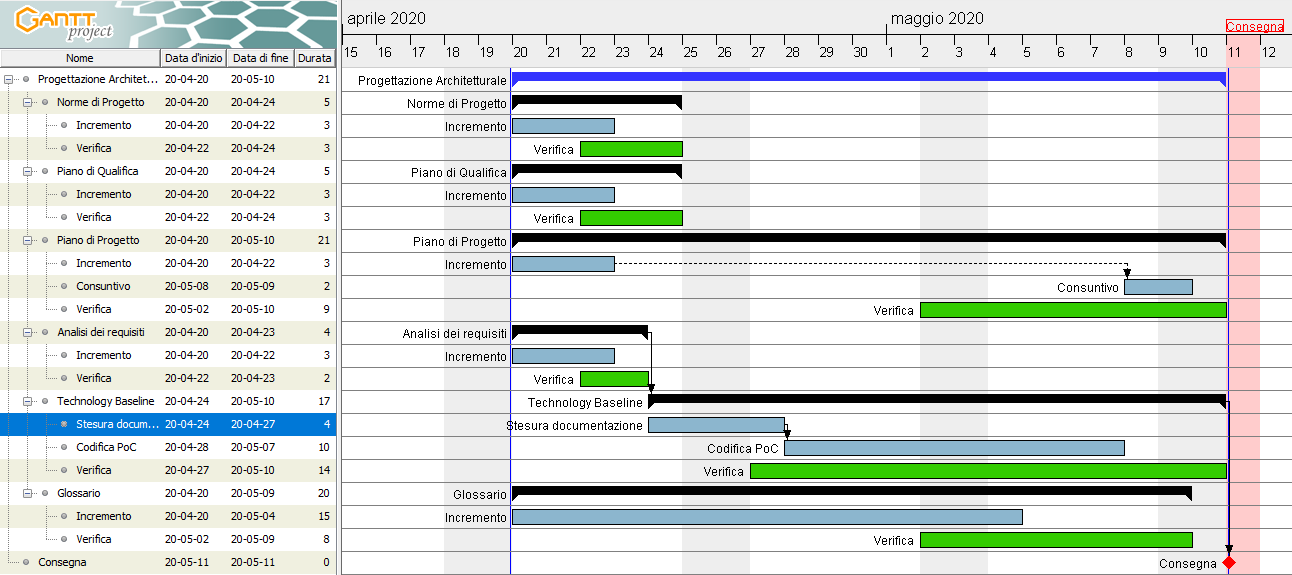
\includegraphics[width=1.1\textwidth]{./res/img/DiagrammiGantt/prog_arch_gantt.png}
			\caption{Diagramma di Gantt del periodo di Progettazione Architetturale}
		\end{figure}
\newpage

\subsection{Progettazione di Dettaglio e Codifica}
\textbf{Periodo}: dal 2020-05-11 al 2020-06-18 \\
Questo periodo ha inizio dopo il termine del periodo di Progettazione Architetturale e termina con la \textit{Revisione di Qualifica}. \\

Le principali attività svolte in questo periodo sono:
\begin{itemize}
	\item \textbf{Incremento e verifica}: come prima cosa, analizzando l'esito della \textit{Revisione dei Progettazione} vengono svolte attività di incremento e verifica sui vari documenti redatti;
	\item \textbf{Product Baseline}\ped{\textit{G}}: progettazione dettagliata a basso livello delle componenti del prodotto\ped{\textit{G}}, coerente con quanto individuato nella \TB{}\ped{\textit{G}}:
	\begin{itemize}
		\item \textbf{Allegato Tecnico}: stesura del documento di \textit{Allegato Tecnico 1.0.0}, di supporto alla progettazione di dettaglio;
		\item \textbf{Codifica}: attività nelle quali viene prodotto e verificato il codice.
	\end{itemize}
	\item \textbf{User Manual} (manuale utente): attività nella quale viene redatto lo \textit{User Manual 1.0.0} contenente le informazioni su come funziona e su come si utilizza il prodotto\ped{\textit{G}};
	\item \textbf{Glossario}: attività che prevede un miglioramento del \textit{Glossario 2.0.0} aggiungendo nuovi termini oppure raffinando le definizioni di termini già presenti.
\end{itemize}

Abbiamo provveduto a dividere il periodo di Progettazione di Dettaglio e Codifica in due sotto-periodi al fine di rendere più agevole e definita la produzione. I sotto-periodi in questione sono:
\begin{itemize}
	\item \textbf{periodo di individuazione dell'architettura e rielaborazione:} in questo periodo sono state attuate le scelte architetturali volte a definire la \textit{Product Baseline} ed è stato rielaborato il codice già esistente secondo l'architettura scelta;
	\item \textbf{periodo di codifica delle nuove funzionalità:} in questo periodo sono state sviluppate le mancanti funzionalità obbligatorie.
\end{itemize}

\subsubsection{Incrementi}
Complessivamente, gli incrementi applicati nel corso di questo periodo (siano essi nuovi oppure solamente raffinati) risultano essere i seguenti:

\subsubsubsection*{Periodo di individuazione dell'architettura e rielaborazione}
\begin{itemize}
	\item \textbf{9$^{\circ}$ Incremento:} correzione dei documenti a seguito delle conoscenze acquisite nei periodi precedenti;
	\item \textbf{10$^{\circ}$ Incremento:} scelta dell'architettura da applicare al prodotto software;
	\item \textbf{11$^{\circ}$ Incremento:} adattamento delle componenti già sviluppate secondo l’architettura scelta;
\end{itemize}

\subsubsubsection*{Periodo di codifica delle nuove funzionalità}
\begin{itemize}
	\item \textbf{12$^{\circ}$ Incremento:} implementazione della funzionalità di rilascio di una funzione (corrispondente al comando \texttt{etherless deploy});
	\item \textbf{13$^{\circ}$ Incremento:} implementazione della funzionalità di eliminazione di una funzione (corrispondente al comando \texttt{etherless delete});
	\item \textbf{14$^{\circ}$ Incremento:} implementazione delle funzionalità per ottenere informazioni su una o più funzioni (corrispondenti ai comandi \texttt{etherless info} e \texttt{etherless list});
	\item \textbf{15$^{\circ}$ Incremento:} stesura dei seguenti documenti:
	\begin{itemize}
		\item stesura dello \textit{User Manual 0.1.0};
		\item stesura del \textit{Developer Manual 0.1.0};
	\end{itemize}
	aggiornamento della documentazione, con corrispondente passaggio alla versione 3.0.0:
	\begin{itemize}
		\item consuntivo di periodo nel \textit{\PdP{}};
		\item valori delle metriche registrati nel \textit{\PdQ{}};
		\item contenuto del \textit{Glossario}.
	\end{itemize}
	\item \textbf{16$^{\circ}$ Incremento:} preparazione della presentazione per la RQ e conseguente raffinamento della demo.
\end{itemize}

Conseguentemente, le scadenze dei vari incrementi sono state ridefinite secondo il seguente calendario:
\begin{itemize}
	\item \textbf{9$^{\circ}$ Incremento:} entro 2020-05-22;
	\item \textbf{10$^{\circ}$ Incremento:} entro 2020-05-26;
	\item \textbf{11$^{\circ}$ Incremento:} entro 2020-05-29;
	\item \textbf{12$^{\circ}$ Incremento:} entro 2020-06-02;
	\item \textbf{13$^{\circ}$ Incremento:} entro 2020-06-04;
	\item \textbf{14$^{\circ}$ Incremento:} entro 2020-06-06;
	\item \textbf{15$^{\circ}$ Incremento:} entro 2020-06-11;
	\item \textbf{16$^{\circ}$ Incremento:} entro 2020-06-18.
\end{itemize}

\subsubsection{Diagramma di Gantt: Progettazione di Dettaglio e Codifica}
	\begin{figure}[h]
		\centering
		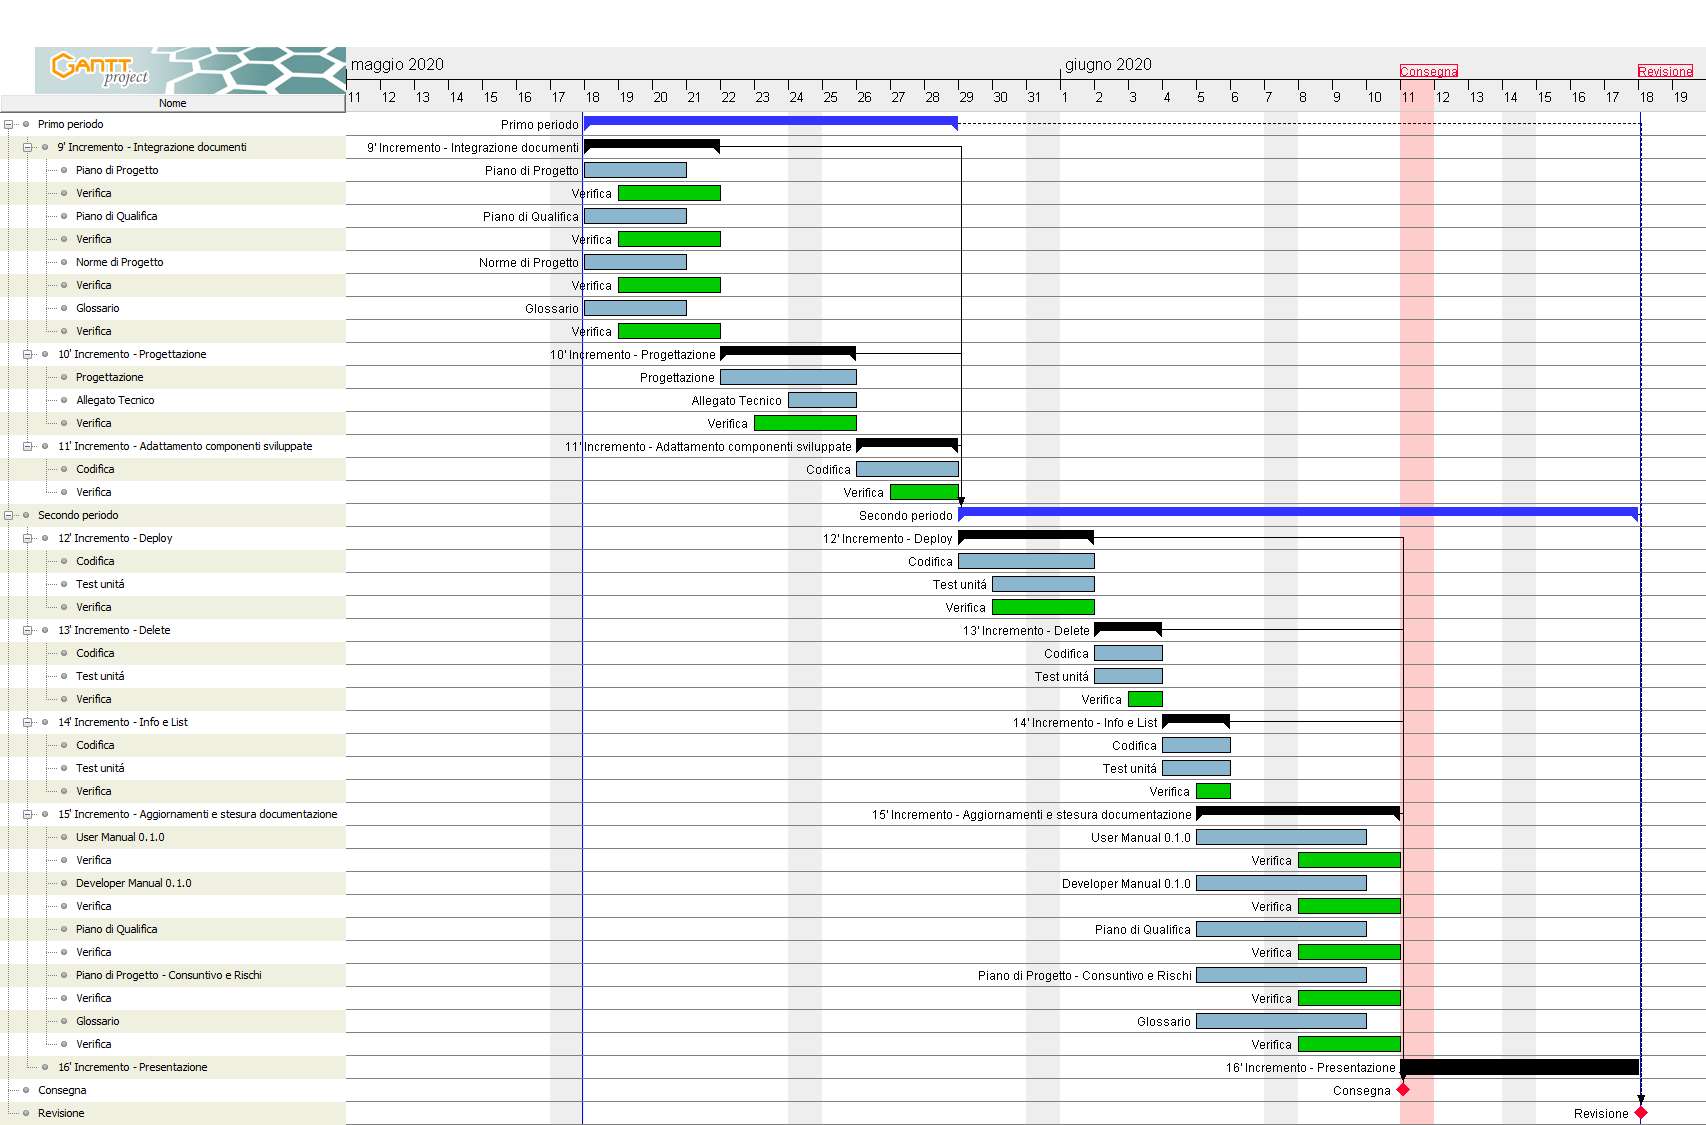
\includegraphics[width=1.1\textwidth]{./res/img/DiagrammiGantt/prog_dett_gantt.png}
		\caption{Diagramma di Gantt del periodo di Progettazione di Dettaglio e Codifica}
	\end{figure}


\newpage

\subsection{Validazione e Collaudo}
\textbf{Periodo}: dal 2020-06-11 al 2020-07-20 \\
Questo periodo ha inizio dopo il termine del periodo di Progettazione di Dettaglio e Codifica, e termina con la \textit{Revisione di Accettazione}. \\
Le principali attività svolte in questo periodo sono:
\begin{itemize}
	\item \textbf{Incremento e verifica}: come prima cosa, analizzando l'esito della \textit{Revisione di Qualifica} vengono svolte attività di incremento e verifica sui vari documenti redatti;
	\item \textbf{Validazione e Collaudo}: attività nella quale vengono eseguiti test e, se necessario, vengono apportati dei miglioramenti al prodotto\ped{\textit{G}} per poter assicurare il soddisfacimento dei requisiti e dei vincoli qualitativi;
	\item \textbf{User Manual}: attività nella quale viene migliorato lo \textit{User Manual 1.0.0};
	\item \textbf{Developer Manual}: attività nella quale viene redatto il \textit{Developer Manual 1.0.0}, il quale contiene le informazioni utili al mantenimento del prodotto\ped{\textit{G}};
	\item \textbf{Glossario}: attività che prevede un miglioramento del \textit{Glossario 3.0.0} aggiungendo nuovi termini oppure raffinando le definizioni di termini già presenti.
\end{itemize}
	\subsubsection{Incrementi}
		\subsubsubsection{Descrizione}
			\begin{itemize}
				\item \textbf{17$^{\circ}$ Incremento:} correzione e integrazione dei documenti a seguito delle conoscenze acquisite nei periodi precedenti e dalla correzione della RQ;
				\item \textbf{18$^{\circ}$ Incremento:} ampliamento del modulo \textit{etherless-cli} mediante l'implementazione dei seguenti comandi:
					\begin{itemize}
						\item init;
						\item whoami;
						\item search.
					\end{itemize}
				\item \textbf{19$^{\circ}$ Incremento:} implementazione del comando history;
				\item \textbf{20$^{\circ}$ Incremento:} implementazione del comando edit;
				\item \textbf{21$^{\circ}$ Incremento:} ampliamento dei test di sistema ed eventuali correzioni necessarie;
				\item \textbf{22$^{\circ}$ Incremento:} aggiornamento della documentazione e stesura del \textit{Developer Manual 1.0.0};
				\item \textbf{23$^{\circ}$ Incremento:} preparazione della presentazione per la RA.
			\end{itemize}
		\subsubsubsection{Scadenze}
			\begin{itemize}
				\item \textbf{17$^{\circ}$ Incremento:} entro 2020-06-24;
				\item \textbf{18$^{\circ}$ Incremento:} entro 2020-06-26;
				\item \textbf{19$^{\circ}$ Incremento:} entro 2020-06-28;
				\item \textbf{20$^{\circ}$ Incremento:} entro 2020-07-03;
				\item \textbf{21$^{\circ}$ Incremento:} entro 2020-07-08;
				\item \textbf{22$^{\circ}$ Incremento:} entro 2020-07-13;
				\item \textbf{23$^{\circ}$ Incremento:} entro 2020-07-20.
			\end{itemize}

	\subsubsection{Diagramma di Gantt: Validazione e Collaudo}
		\begin{figure}[h]
			\centering
			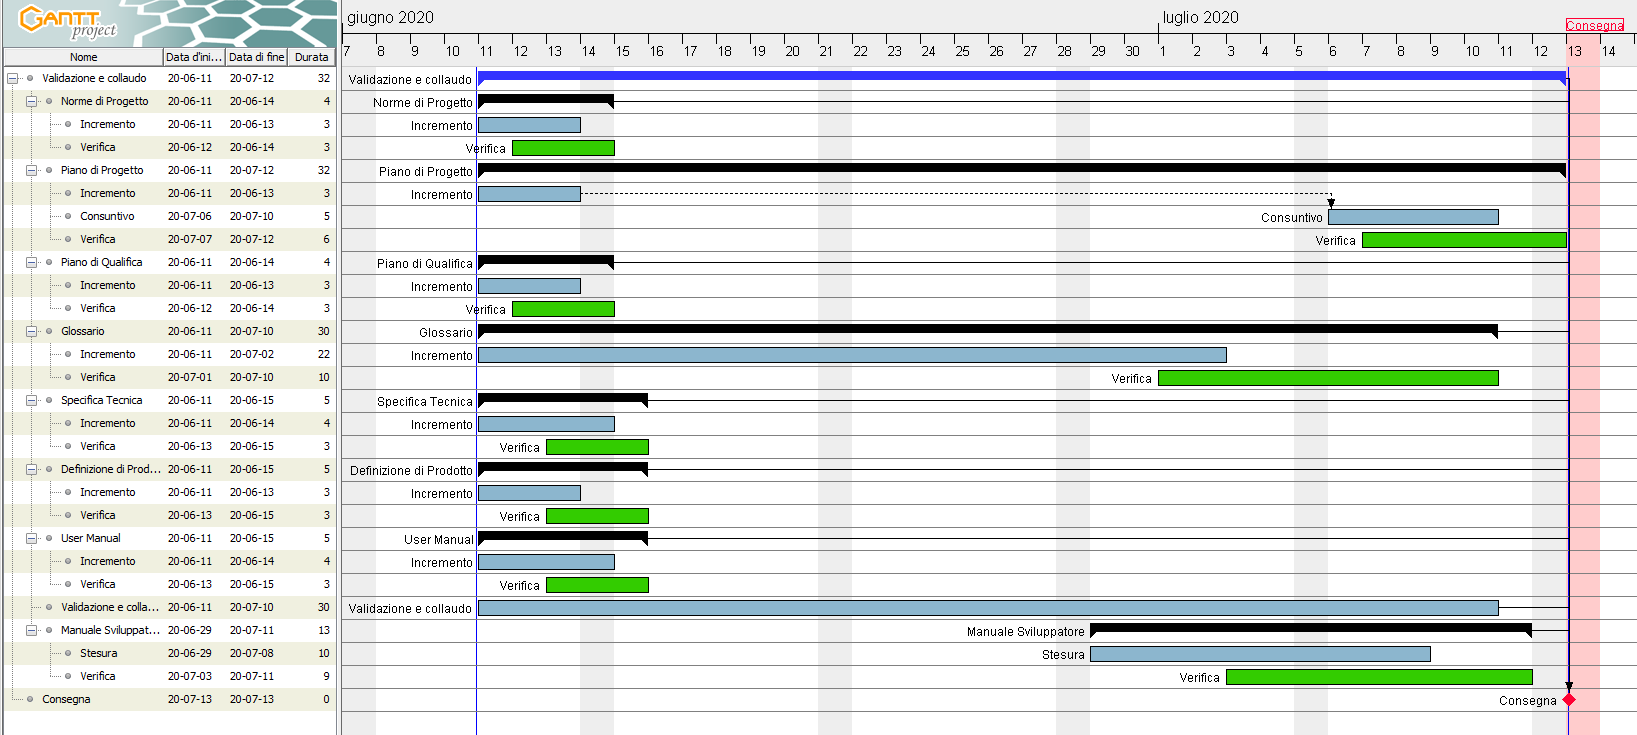
\includegraphics[width=1.1\textwidth]{./res/img/DiagrammiGantt/validaz_gantt.png}
			\caption{Diagramma di Gantt del periodo di Validazione e Collaudo}
		\end{figure}
